% Aquí contendrán los métodos y procedimientos adoptados en el desarrollo del trabajo. Esta es una de las sesiones más importantes pues demuestra el poder científico que se utilizó para la investigación. Sin una buena metodología la investigación puede perder la validez. El investigador debe utilizar métodos o técnicas aceptadas por la comunidad científica en la búsqueda de probar sus hipótesis.

% La metodología elegida debe ser aquella que más se adecue a su objeto de estudio y al enfoque aplicado. Hay dos métodos principales: 1) cuantitativo, que es el uso de instrumental estadístico, de datos numéricos; y 2) cualitativo, que se caracteriza por la calificación de los datos recogidos, durante el análisis del problema.


\chapter{Web Semántica}
\label{ch:web-semantinca}

\begin{quote}
  {\bf\textsc{Resumen:}} Este capítulo ...
\end{quote}

\section{Web Semántica}

% http://www.fgcsic.es/lychnos/es_es/articulos/construyendo_una_web_semantica
% http://www.bibliopos.es/Biblion-A2-Bibliografia-Documentacion/18ontologia-Web-Semantica.pdf
% https://www.ceupe.com/blog/que-es-la-la-web-semantica.html
% https://disenowebakus.net/semantica-web.php
% http://cmap.javeriana.edu.co/servlet/SBReadResourceServlet?rid=1264791321546_232600024_2804
% https://www.w3c.es/Eventos/2009/Talleres/Murcia/Presentaciones/jesualdo.pdf
% https://www.wiziq.com/tutorial/143922-La-Web-Semantica-y-sus-Principales-Caracteristicas
% http://personales.upv.es/ccarrasc/doc/2002-2003/WebSem/WS_2_b.htm
% http://inteligencia-artificial-unsxx.blogspot.com/p/web-semantica-y-web-30.html

% https://www.weblaspalmas.es/noticias-tecnologicas/172/La-web-3-0-De-la-web-social-a-la-semantica.html

% https://wiki.dbpedia.org/

%  Web 3.0: integración de la Web Semántica y la Web 2.0:  http://www.albertolsa.com/wp-content/uploads/2009/07/redessociales-web-30-integracion-de-la-web-semantica-y-la-web-20-los-santos-nava-godoy.pdf

% evolucion de la web: http://profesores.elo.utfsm.cl/~tarredondo/info/networks/Evolucion_Web.pdf

% aplicación de la web semántica en tráfico: https://www.ptcarretera.es/wp-content/uploads/2018/07/02_2017_lisitt_def.pdf

% hablar sobre los tipos de web, según veo hay Web 1.0, Web 2.0 y Web 3.0 o Semántica

% CURSO EN COURSERA INTERESANTE: https://es.coursera.org/learn/web-semantica?action=enroll

% http://www.mclibre.org/consultar/xml/lecciones/web-semantica.html

% Las web 3.0: de la web social a la semántica: https://www.puromarketing.com/12/15656/social-semantica.html

La Web Semántica permitirá a las máquinas comprender documentos y datos semánticos, pudiendo asÍ colaborar entre ellas y con las personas.\\

La Web Semántica no es una Web aparte, es una extensión de la Web actual que permite que los datos tengan un significado bien definido, de manera que personas y ordenadores puedan trabajar en cooperación más fácilmente.

% tengo que ver como meter el apartado de 1.4 del Capítulo 1 

Por web semántica se entiende una forma de organizar el contenido en la Web que mejore la cooperación entre computadoras y humanos. Esto pasa por avanzar de una web de documentos a una web de datos enlazados en la que se puedan ofrecer novedosos servicios que hagan uso del potencial de combinar e interrelacionar datos de diversa índole y procedencia.


% COURSERA

 ¿Y cómo es la web actual? Primero la web actual es masiva. ¿Cuántos millones y millones de páginas web existen? Además la web actual es cambiante ¿Cuántos tweets por segundo se generan? ¿Cuántas actualizaciones de perfil de Facebook se generan? Incontables, además la web actual es heterogénea ¿Cuántos millones de dispositivos como éste, o como sensores generan datos? La web actual además es distribuida, cualquier persona en el mundo puede acceder o generar contenido, no solo esto la web actual es un gran repositorio de información al cual todo el mundo puede acceder.
 
 ¿Pero es realmente accesible esta información? Hoy en idea tenemos herramientas como Google y Bing y muchas otras que nos dan acceso a los datos. Pero estas herramientas tienen dificultades al momento de entender la información que está contenida en ellos. En particular estas herramientas miran las páginas web como si fueran conjunto de palabras, y no son capaces de entender o tienen dificultades al momento de entender los distintos elementos que forman parte de ella, que pueden ser tan diversos como personas, lugares geográficos, publicaciones, películas etcétera, y además tienen dificultades al momento de entender las relaciones que existen entre estos elementos.
 
 En este curso verá en que consisten las tecnologías de la Web Semántica y como se utilizan en la web actual. También tendrá la oportunidad de realizar varios proyectos aplicando todas estas tecnologías para resolver los problemas que Marcelo ha comentado anteriormente. Por ejemplo, ¿le gustaría que Google entendiera cada uno de los componentes de su página web? O si usted tienen una tienda virtual, ¿le gustaría que Google fuera capaz de identificar los distintos productos que forman parte de su tienda virtual y los desplegara al momento de hacer una búsqueda? Esto se consigue usando [DESCONOCIDO] y les mostraremos como se relaciona en este curso con las tecnologías de la Web Semántica.
 
 Además, ¿le gustaría poder acceder a la Wikipedia como si fuera una tabla Excel? ¿O le gustaría poder conocer como han hecho los gobiernos para hacer públicos sus datos y de esta manera permitir que los ciudadanos puedan acceder a la información de como se gastan sus impuestos, o puedan entender de una manera más sencilla como le afecta una ley? ¿O le gustaría saber como hacen los biólogos para compartir sus datos en la web?
 
 \section{La web actual y sus desafíos}
 
 La web semántica es lo que va a ser la web del futuro. Pero para poder llegar a la web del futuro tenemos que entender cuál es la web actual en la que estamos. Entonces, la web actual en la que estamos está compuesta por documentos. Estos documentos son básicamente páginas web html que vemos cualquier día, todos los días en nuestro navegador web. Estos documentos web están compuestos por contenido, que pueden ser texto, pueden ser imágenes, pueden ser vídeos, audios, etcétera. Y además está compuesto por enlaces. Estos enlaces nos llevan a otras páginas web. Esta es la forma de la web actual. Es la que todos conocemos.
 
 [ejemplo arquitectura de como funciona la web actual]
 
  Todos estamos bastante familiarizados con la Web y sobre cómo operar con ella. Abrimos un navegador (por ejemplo, Explorer, Firefox o Safari) e introducimos la dirección de la página que deseamos consultar o bien pedimos a un buscador (por ejemplo Google o Yahoo!) que nos determine las ubicaciones de documentos en la Web que contengan una combinación de palabras deseada y que nos las ordene por importancia.­ % http://www.fgcsic.es/lychnos/es_es/articulos/construyendo_una_web_semantica
 
 Un ejemplo de esta web actual sería el que vemos ahora en la pantalla. Este ejemplo lo que contiene es la descripción de la world wide web en la Wikipedia. Todos conocemos la Wikipedia y es muy sencillo acceder a ella. Dentro de esa descripción podemos ver que tenemos texto. Mucho texto. Esto sería principalmente el contenido de la página web. Además tenemos una imagen dentro de esta página web. Sería una parte más del contenido de la página web. Además, dentro de esta página web de la Wikipedia tenemos enlaces. Por ejemplo, tenemos enlaces a informática, tenemos enlaces a computación, tenemos enlaces a Internet. Estos enlaces nos redirigen a otra página web con un contenido distinto.
 

 
 [ejemplo de una página web]
 
 % mencionar algo de pubmed
 
 Seguimos hablando de enlaces. Y los enlaces en este otro ejemplo son enlaces de PubMed. PubMed es una base de datos. Una página web que contiene documentos científicos, documentos médicos sobre enfermedades y demás. Entonces aquí tenemos varios ejemplos de enlaces que nos llevan, precisamente, a esos documentos científicos de medicina.
 
 
 Entonces ya hemos visto un poquito como es la web actual y ahora vamos a ver los desafíos que presenta esta web actual. El primer desafío es la heterogeneidad. Como hemos visto, la Wikipedia tiene un formato, PubMed tiene otro formato, Facebook tiene otro formato de datos, nos presenta las cosas de forma distinta. Es decir la web es muy heterogénea.
 
\begin{figure}[H]
	\centering
	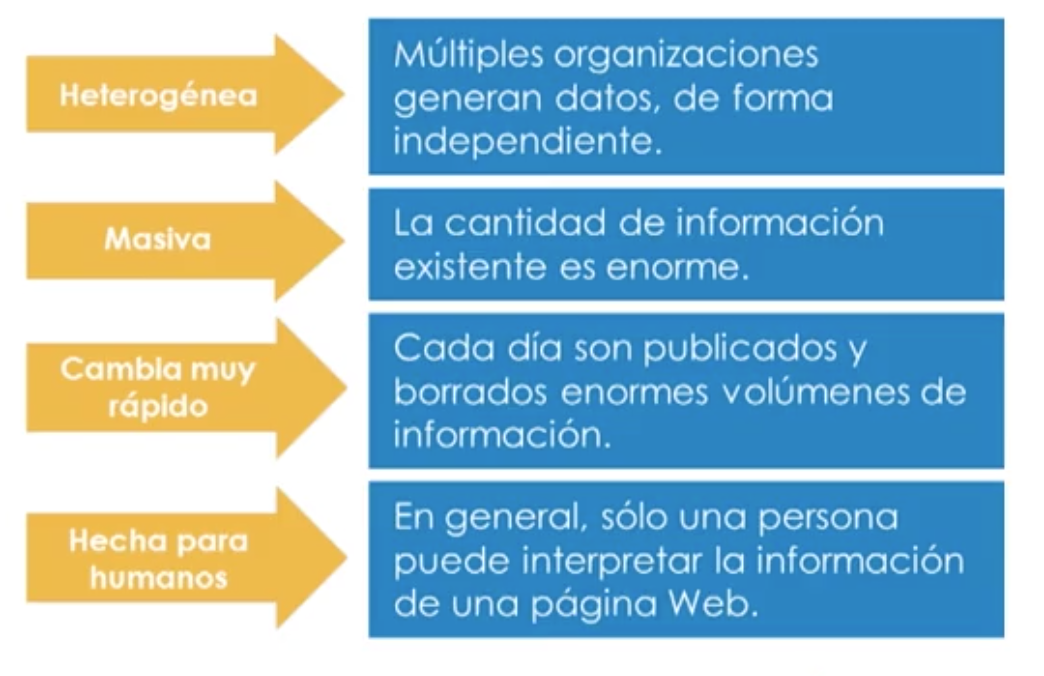
\includegraphics[height=4.5cm]{imagenes/capitulo3/1}
	\caption{}
\end{figure}
 
 
 
 Además la web es masiva. Hay muchísimos datos en PubMed, en Wikipedia, en Facebook. Hay una cantidad ingente de datos. Además cambia muy rápido. Por ejemplo, yo podría estar actualizando mi perfil de Facebook cada hora, cada dos horas. Hay gente que lo actualiza cada 15 minutos. Entonces todo esto cambia muy rápido y estoy dando un ejemplo muy chiquito, muy concreto.
 
 Y sobre todo, la web actual está hecha para humanos. Si nos hemos fijado hasta el momento, los ejemplos que he puesto, la Wikipedia, PubMed Facebook, todo esto está hecho para que sea consumido por humanos. Las máquinas, el software no tiene tanto acceso a este contenido. Es difícil para un programa interpretar los datos que hay, por ejemplo, en el perfil de Facebook de una persona. o dentro de la Wikipedia.
 
 \begin{figure}[H]
 	\centering
 	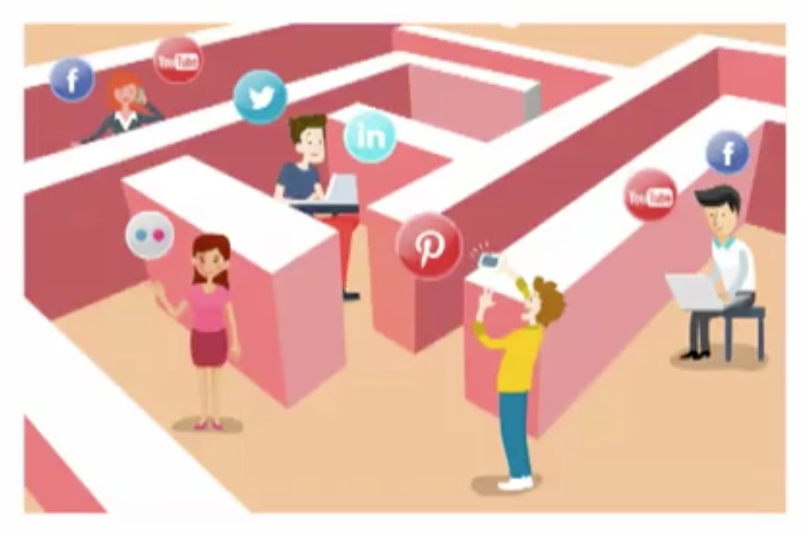
\includegraphics[height=4.5cm]{imagenes/capitulo3/2}
 	\caption{}
 	\label{}
 \end{figure}
 
 
 
 
 Más en detalle la web es heterogénea porque cada aplicación web, cada página web crea los datos y los presenta a los usuarios de una forma totalmente distintas. Es distinto lo que se hace en Facebook, en LinkedIn, en Orkut, en MySpace. Todas esas son redes sociales. Son totalmente distintas y no intercambian datos entre ellas.
 
 Además la web es masiva. Por ejemplo, la Wikipedia son casi 6 terabytes de datos. Y ¿qué es un terabyte de datos?
 
 En un terabyte de datos caben 678 millones de páginas de texto. 678 millones, eso, suponiendo que el Quijote tiene 1.000 páginas de texto, quiere decir que en un terabyte caben 678 mil Quijotes, Y en una Wikipedia, con 6 terabytes de datos, caben alrededor de 4 millones de Quijotes. Muchísimo.
 
 La web actual cambia muy rápido. Actualmente se transfieren en Internet 160 terabytes de datos por segundo. Esos son 27 Wikipedias por segundo. Se transfieren alrededor de Internet 27 Wikipedias cada segundo. Eso es muchísimo.
 
 Además la web está hecha para humanos. Como comentaba anteriormente Facebook lo consumen principalmente las personas. La Wikipedia la consumen normalmente las personas. Pero ¿qué pasa si yo quiero enlazar o combinar los datos de la Wikipedia y de Facebook o la Wikipedia y de PubMed? Eso actualmente, con el diseño de la web actual no es posible.
 
 Entonces ¿cómo podría una aplicación consumir datos de dos webs distintas? Leyendo el texto, el contenido. Pero, ¿cómo sabe qué texto leer? ¿Cómo sabe qué contenido leer dentro de una página web?
 
 Mirando el código de la html de cada página web. Podría ser pero es muy desordenado. Por dentro el código está muy desordenado siempre. Uno no sabe, una aplicación no sabría exactamente dónde está el nombre de una persona dentro del código html. Normalmente es muy difícil de saber.
 
  \begin{figure}[H]
 	\centering
 	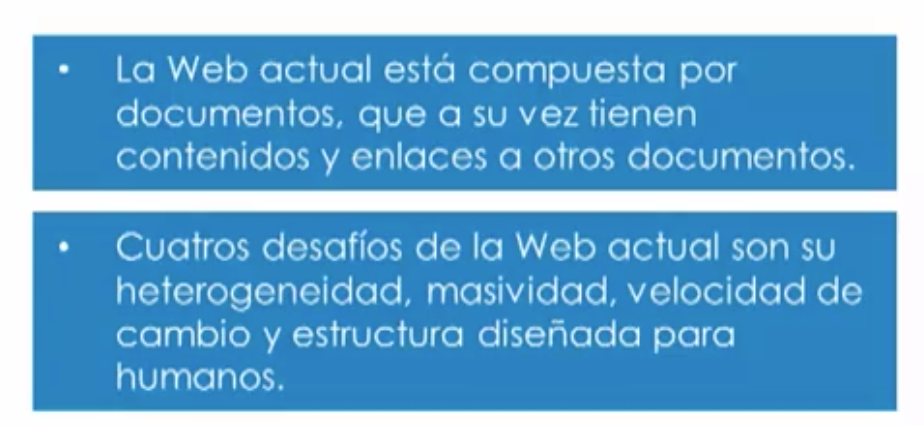
\includegraphics[height=4.5cm]{imagenes/capitulo3/3}
 	\caption{}
 \end{figure}

Entonces, para resumir hemos visto que la web es masiva, está compuesta por documentos. Estos documentos tienen contenido y enlaces a otras páginas web. Hay varios desafíos dentro de la web actual que son la heterogeneidad, la velocidad de cambio, la masividad de la web. Y que está hecha para humanos. Un software, una aplicación no sabe identificar o consumir los datos de una página web.

Entonces, estos son los desafíos que intenta resolver la web semántica. Sobre todo la parte de la heterogeneidad de datos y la parte de que está hecha para los humanos. La web semántica va a tratar de derribar las barreras que existen en la web actual para que los contenidos puedan ser consumidos por máquinas de manera mucho más eficiente.



\begin{figure}[H]
	\centering
	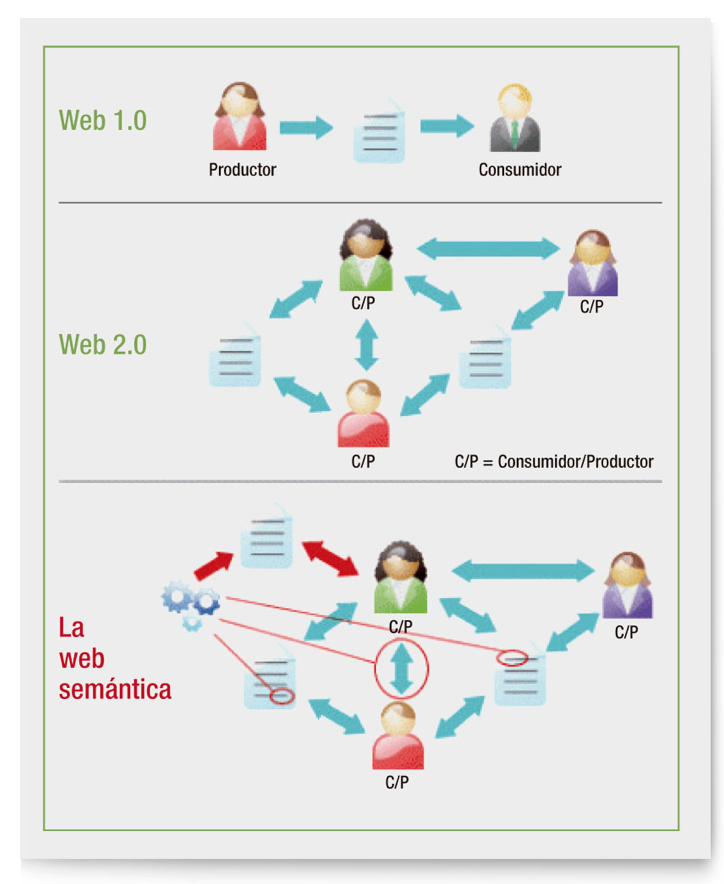
\includegraphics[height=4.5cm]{imagenes/capitulo3/10}
	\caption{}
\end{figure}
% Evolución de una web cuyo contenido es producido por unos y consumidos por otros a una web semántica que mejora la cooperación entre computadoras y humanos.

A partir de ahí podemos ir saltando de una página web a otra a través de hipervínculos –estas palabras, frases, imágenes o iconos que generan la descarga automática de otra página web cuando pinchamos sobre ellos–. Esto es lo que se conoce como la web de primera generación o Web 1.0: personas con conocimiento especializado de diseño y composición de páginas web crean los documentos con su contenido y definen los hipervínculos que los entrelazan; los usuarios no expertos son fundamentalmente consumidores de información. Leen noticias, consultan diccionarios, visualizan imágenes o vídeos o compran productos. % http://www.fgcsic.es/lychnos/es_es/articulos/construyendo_una_web_semantica

En la web de segunda generación, la Web 2.0, los usuarios no expertos, además de consumidores, pueden ser también generadores de contenidos y proveedores de servicios. Mediante blogs, por ejemplo, se pueden escribir y compartir reflexiones periódicas, y los lectores pueden añadir comentarios o nuevos enlaces relevantes; con Wikipedia, millones de personas construyen una gran enciclopedia multilingüe que constantemente es actualizada y ampliada por los propios usuarios; a través de redes entre pares, como originalmente Napster, BitTorrent o eMule, se comparten películas y ficheros de música; y últimamente, con la irrupción de las redes sociales —Facebook, Tuenti o Twitter—, la Web se ha convertido en un espacio global de participación e interacción entre usuarios.% http://www.fgcsic.es/lychnos/es_es/articulos/construyendo_una_web_semantica

La web semántica viene a ser la tercera generación de la Web, la Web 3.0, una extensión de la Web actual en la que los contenidos están organizados de forma que no solo los humanos sino también las computadoras sean capaces de procesar su significado —por eso lo de semántica— posibilitando así una mejor cooperación entre computadoras y humanos. La nomenclatura Web 1.0, 2.0 y 3.0 es seguramente artificiosa, ya que de hecho no se trata de nuevas versiones de la Web, sino de la misma web de siempre pero con niveles añadidos de funcionalidad. % http://www.fgcsic.es/lychnos/es_es/articulos/construyendo_una_web_semantica


 
 
\subsection{Web actual vs. Web Semántica}

La mayoría de los contenidos de la Web actual están diseñados para ser leídos por humanos.

Los ordenadores puede analizar la estructura de las páginas Web y determinar cuál es la cabecera, dónde hay un enlace a otra página, etc.

- No tienen una forma fiable de procesar la semántica de las páginas.

La Web Semántica proporciona estructura al contenido semántico de las páginas Web, para que puedan ser tratadas por máquinas.

– Crea un entorno donde los agentes que vagan de página a página pueden realizar tareas sofisticadas para los usuarios: no sÓlo miran las palabras clave de las páginas, sino que recogen la semántica de los datos.

Todo ello “sin Inteligencia Artificial”, la semántica está en las páginas. 

– Además, las páginas han sido desarrolladas por usuarios “no informáticos”.

% diagrama de web y diagrama de web semántica

% deberíamos de hablar algo sobre la web

% estaría bien decir que signfica semántica por un lado, que signfica sintáctico por otro y así ir uniendo
% búsquedas semánticas, no sólo sintácticas.

% mencionar algo sobre lo de interoperabilidad

% hablar sobre OGC

% hablar sobre HTML y XML

\section{De una web de documentos a una web de datos}

Para alcanzar esta visión de una web semántica de entrada no se deberían enlazar únicamente documentos de texto, imágenes u otro contenido multimedia sino directamente los datos sin procesar.% http://www.fgcsic.es/lychnos/es_es/articulos/construyendo_una_web_semantica

El conjunto de buenas prácticas para la publicación y el enlace de datos estructurados en la Web se conoce como Linked Data, datos enlazados. He aquí sus puntos principales:

% http://www.fgcsic.es/lychnos/es_es/articulos/construyendo_una_web_semantica

- Cada dato –o cada recurso, como suele llamarse a la información en la Web– debe tener un identificador único que lo distingue de cualquier otro dato publicable en la Web. Es lo que se conoce como Universal Resource Identifier, o URI. De hecho muchos usuarios de la Web ya estamos familiarizados con lo que es un URI. Por ejemplo, la dirección https://www.cia.gov/library/publications/the-world-factbook/geos/sp.html es el URI que identifica la página web con la información sobre España en el World Factbook. Pero, para enlazar datos, los URI deben identificar no solo a páginas sino a los elementos concretos que componen los datos. Así, pues, para publicar el hecho de que España y Francia compartan frontera debemos tener unos URI que identifiquen «España», «comparte frontera con» y «Francia», respectivamente.

- Al mismo tiempo, estos identificadores deben ser desreferenciables, lo que significa que el identificador del recurso apunta a su vez al lugar en la Web donde podemos acceder al mismo. La desreferencia de un URI (literalmente «deshacer la referencia») se realiza mediante el protocolo HTTP (Hypertext Transfer Protocol) que posibilita los hipervínculos en la Web: cuando pinchamos sobre uno de estos vínculos, el protocolo HTTP toma el URI y a través de él es capaz de acceder al contenido al cual está apuntando. Lo mismo debe ocurrir ahora con los recursos que componen un dato. El URI de «comparte frontera con» deberá poder ser desreferenciado para acceder a la definición de lo que significa esta relación. Ahí entra la semántica: disponer de estas definiciones y poder acceder a ellas.

- Los datos propiamente dichos se deben expresar usando el Resource Description Framework o RDF, un lenguaje para estructurar los datos en enunciados con el simple formato sujeto-predicado-objeto, y que se conoce como triplete. El sujeto y el objeto son recursos identificados mediante un URI, y el predicado es la relación entre estos recursos. Así pues el hecho de que España comparte frontera con Francia se expresaría en forma de triplete RDF de la siguiente manera:

sujeto: %http://www4.wiwiss.fu-berlin.de/factbook/resource/Spain
predicado: %http://www4.wi­wiss.fu-berlin.de/factbook/ns#landboundary
objeto: %http://www4.wiwiss.fu-berlin.de/factbook/resource/France

Hemos usado las URI de la publicación del World Factbook como Linked Data realizada por la Universidad Libre de Berlín. Como se puede observar, en RDF la relación entre sujeto y objeto –el predicado– es a su vez también un recurso con su URI que debe ser desreferenciable. Como hemos dicho anteriormente, es así como accederemos a sus definiciones, especificando por ejemplo que Spain y France son países y que landboundary es la relación de dos países que comparten una frontera. Estas definiciones que aquí hemos expresado en lenguaje natural deberían ser especificadas a su vez como datos publicados en forma de tripletes RDF.

- Finalmente, para poder utilizar todo el potencial que nos ofrece la infraestructura de la Web, los datos de un repositorio o base de datos deberían estar enlazados con datos externos, definidos en otro repositorio o base de datos. Es decir, el sujeto, predicado y objeto de un mismo triplete RDF no tienen por qué estar ubicados, definidos y gestionados en el mismo repositorio de datos, sino que pueden estar distribuidos por la Web.

Publicando los datos directamente en formato RDF, con unos URI desreferenciables que apuntan a definiciones de entidades y sus relaciones, que a su vez se expresan como datos en RDF enlazando así unos datos con otros, es como se añade a la infraestructura tecnológica existente de la Web este nivel, que puede aumentar significativamente su funcionalidad pues permite procesar estos datos y sus relaciones de forma automatizada. Al igual que en la web de documentos, en la web de datos cualquier persona u organización puede publicar datos, del tipo que sea, y definir los vocabularios asociados a recursos y relaciones. Una buena práctica es usar los URI y los vocabularios ya existentes y ampliamente utilizados. A diferencia de la web de documentos, la estructuración de los datos es independiente de su visualización en pantalla para un usuario humano.


\section{Introducción a la Web Semántica}

% COURSERA

Como habíamos visto en el video anterior, hay datos de todo tipo en la web, tenemos datos genéricos, datos médicos, noticias, datos fundamentales. Y en general, estos datos son de fácil acceso de las personas. En general las páginas web están diseñadas para que sean leídas por personas y formatos adecuados para que las personas puedan acceder a la información. Pero tenemos un problema, la cantidad de datos es tan grande que no la podemos manejar. Solo piensa en los datos que a los cuales usted accede a la web. Por ejemplo tiene el correo electrónico, puede crear una página en Facebook, puede tener información en Instagram, puede acceder a información en Wikipedia y en información general, puede acceder a información geográfica, etcétera, etcétera. ¿Sí? Veamos algunos ejemplos de estos datos en la web. 

 \begin{figure}[H]
	\centering
	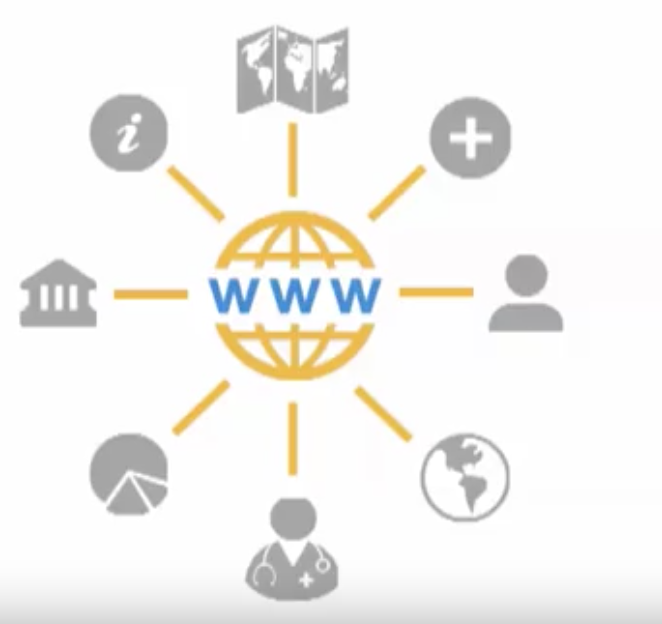
\includegraphics[height=4.5cm]{imagenes/capitulo3/4}
	\caption{}
\end{figure}

 \begin{figure}[H]
	\centering
	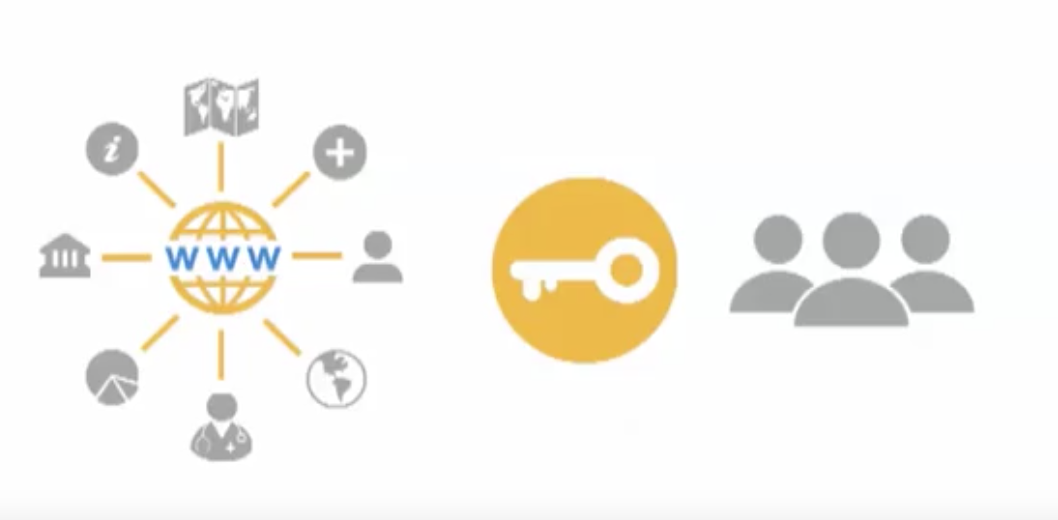
\includegraphics[height=4.5cm]{imagenes/capitulo3/5}
	\caption{}
\end{figure}

 \begin{figure}[H]
	\centering
	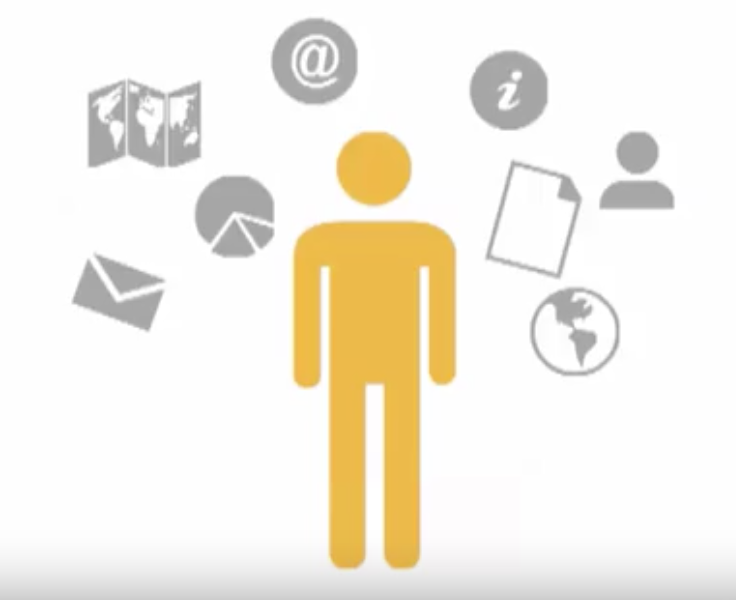
\includegraphics[height=4.5cm]{imagenes/capitulo3/6}
	\caption{}
\end{figure}


En primer lugar tenemos datos genéricos como el ejemplo en Wikipedia. En Wikipedia podemos encontrar información sobre todo tipo de elementos, por ejemplo información geográfica, información sobre historia de los países, información sobre, información científica, etcétera, etcétera. Si bien en algún lugar también tenemos datos médicos, por ejemplo tenemos la biblioteca nacional de medicina de Estados Unidos, donde acá uno puede encontrar información sobre enfermedades, sobre tratamientos, sobre síntomas, etcétera. También tenemos noticias y en esto probablemente usted todos los días lee algún diario que está publicado en la web, por ejemplo The New York Times. También tenemos datos gubernamentales, los distintos gobiernos han decidido tener leyes de transparencia que han obligado a las distintas agencias de estos gobiernos a publicar datos en la web. Por ejemplo, en esta transparencia podemos ver el London Data store, donde la ciudad de Londres guarda información gubernamental, por ejemplo información sobre transporte, sobre salud pública, etcétera.

Entonces, ¿cómo podemos aprovechar estos datos? Algo que es importante tener en cuenta en este momento, es que los computadores tienen la capacidad para poder analizar estos datos, tenemos suficientes computadores, tenemos suficientes procesadores como para organizar esta información. Pero, ¿cuál es el problema que tenemos actualmente? Es que los capaces, los computadores no son capaces de interpretar la información que está en estas páginas web, o sea, las páginas están pensadas para ser leídas por personas no por computadores. Entonces, ¿qué es lo que necesitamos hacer? Hay que permitir que las aplicaciones computacionales entiendan los datos. Y aquí la pregunta fundamental es, ¿cómo podemos hacer esto?

Entonces, ¿cuáles son los requisitos para una web de datos efectiva por una web donde los computadores y las personas puedan acceder y entender la información? En primer lugar, es necesario tener un lenguaje que nos permita especificar los recursos que tenemos en la web y cuáles son las relaciones que existen entre ellos. ¿Sí? Con recurso me refiero a los distintos componentes de la web, esto puede ser una página web, un diario, una persona que tiene una página web, etcétera. Y queremos también especificar cuáles son las relaciones que existen entre ellos. Por ejemplo, esta noticia fue publicada en este diario, esta página de aquí, esta página por ejemplo tiene información sobre problemas de salud en este determinado país, etcétera, etcétera. Ahora un requisito fundamental para diseñar este lenguaje que nos permita especificar recursos, sus relaciones es que el debe ser procesable por un computador. Un computador, una aplicación computacional debe entender este lenguaje. En segundo lugar, necesitamos poder consultar estos datos mediante aplicaciones computacionales y con esto nos referimos a poder especificar lo que estamos buscando y que de manera automática se extraiga esta información. Aquí nuevamente tenemos dos requisitos fundamentales, debemos tener un lenguaje para describir consultas que sea procesable por un computador de nuevo vamos a describir una consulta en un cierto lenguaje y lo que esperamos que el computador entienda o la aplicación computacional entienda esta consulta y debemos ser capaz de sacar conclusiones a partir de los datos de manera automáticos. Debemos ser capaces de extraer de manera automática la respuesta a la consulta o la respuesta a las consultas que estamos realizando.

 \begin{figure}[H]
	\centering
	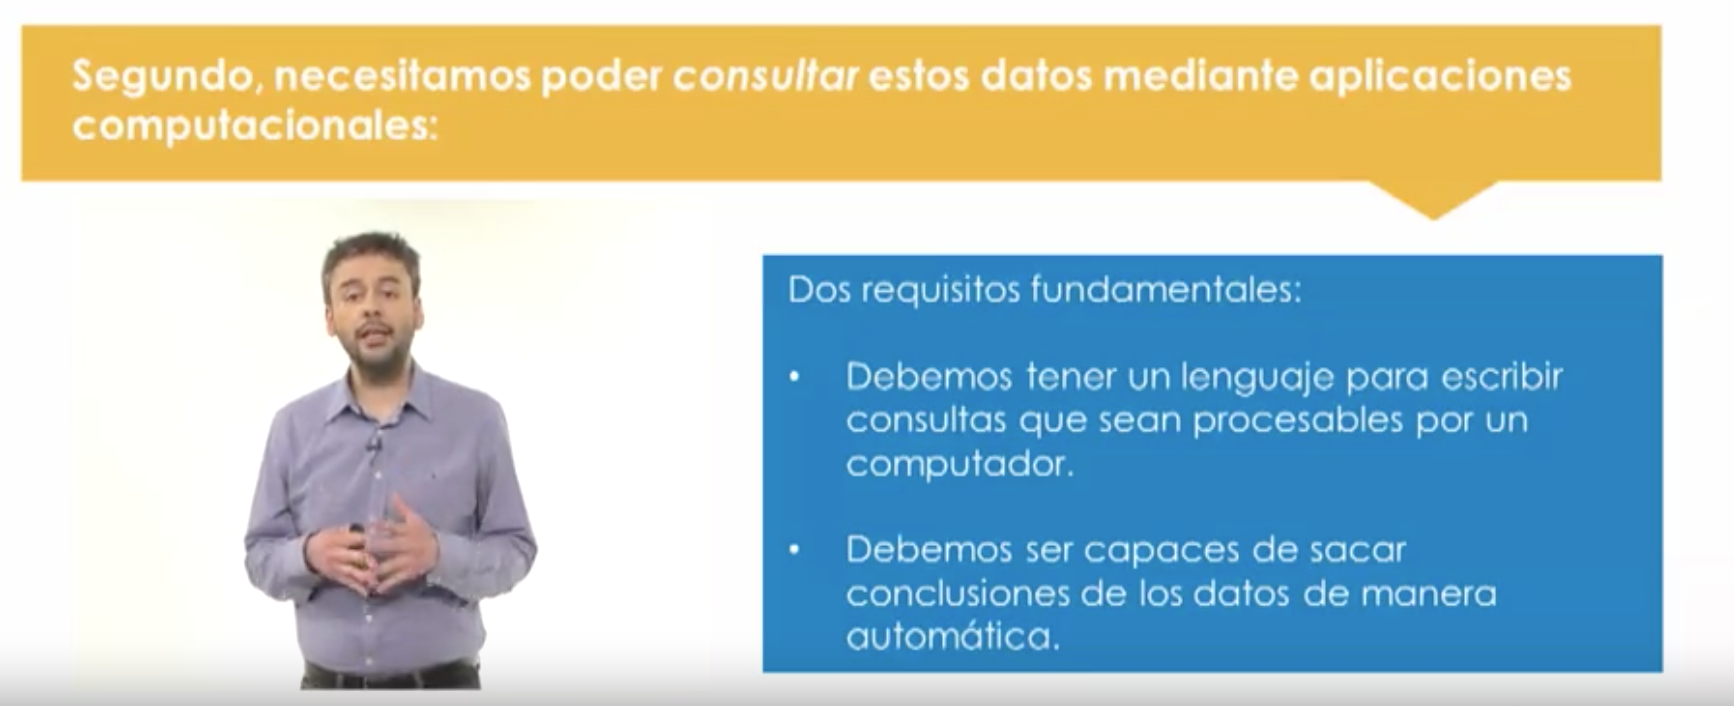
\includegraphics[height=4.5cm]{imagenes/capitulo3/7}
	\caption{}
\end{figure}


En mayo de 2001 la revista Scientific American publicaba un artículo en el que se proponía una nueva forma de organizar el contenido en la Red que desencadenaría una avalancha de posibilidades y, en consecuencia, revolucionaría Internet. El primer autor del artículo era Tim Berners-Lee, el físico del CERN que en 1980 desarrolló un sistema de vinculación y transferencia de documentos en red que acabó convirtiéndose en la World Wide Web que todos conocemos hoy. A la nueva forma de organización de la Web que los autores de dicho artículo pregonaban la llamaron web semántica. % http://www.fgcsic.es/lychnos/es_es/articulos/construyendo_una_web_semantica

En este punto es donde aparece la web semántica en este curso, en palabras de Tim Berners-Lee la web semántica es una extensión de la web actual en la cual se da un significado bien definido a la información, permitiendo mejorar la colaboración entre personas y computadores en la web. ¿En qué se traduce esto en la práctica? Bueno, la web semántica en la práctica lo que vemos hoy en día es un conjunto de recomendaciones desarrolladas por el World Wide Web Consortium, cuyo objetivo es que los computadores sean capaces de entender los datos en la web. Aquí tenemos que detenernos en dos conceptos importantes. En primer lugar, ¿qué es una recomendación? En este nivel, una recomendación es una descripción formal de una tecnología que debería ser utilizada por todos. ¿Sí? Es decir, un lenguaje común para todos. Lo que queremos hacer en este punto es desarrollar un lenguaje que por ejemplo nos permita especificar los recursos de la web que tenga una descripción formal, para que así pueda ser entendida por un computador y que sea un lenguaje común para todos. También es importante mencionar acá que el World Wide Web Consortium es el organismo regulador de la web, es el organismo que dicta los distintos estándares para la web.

 \begin{figure}[H]
	\centering
	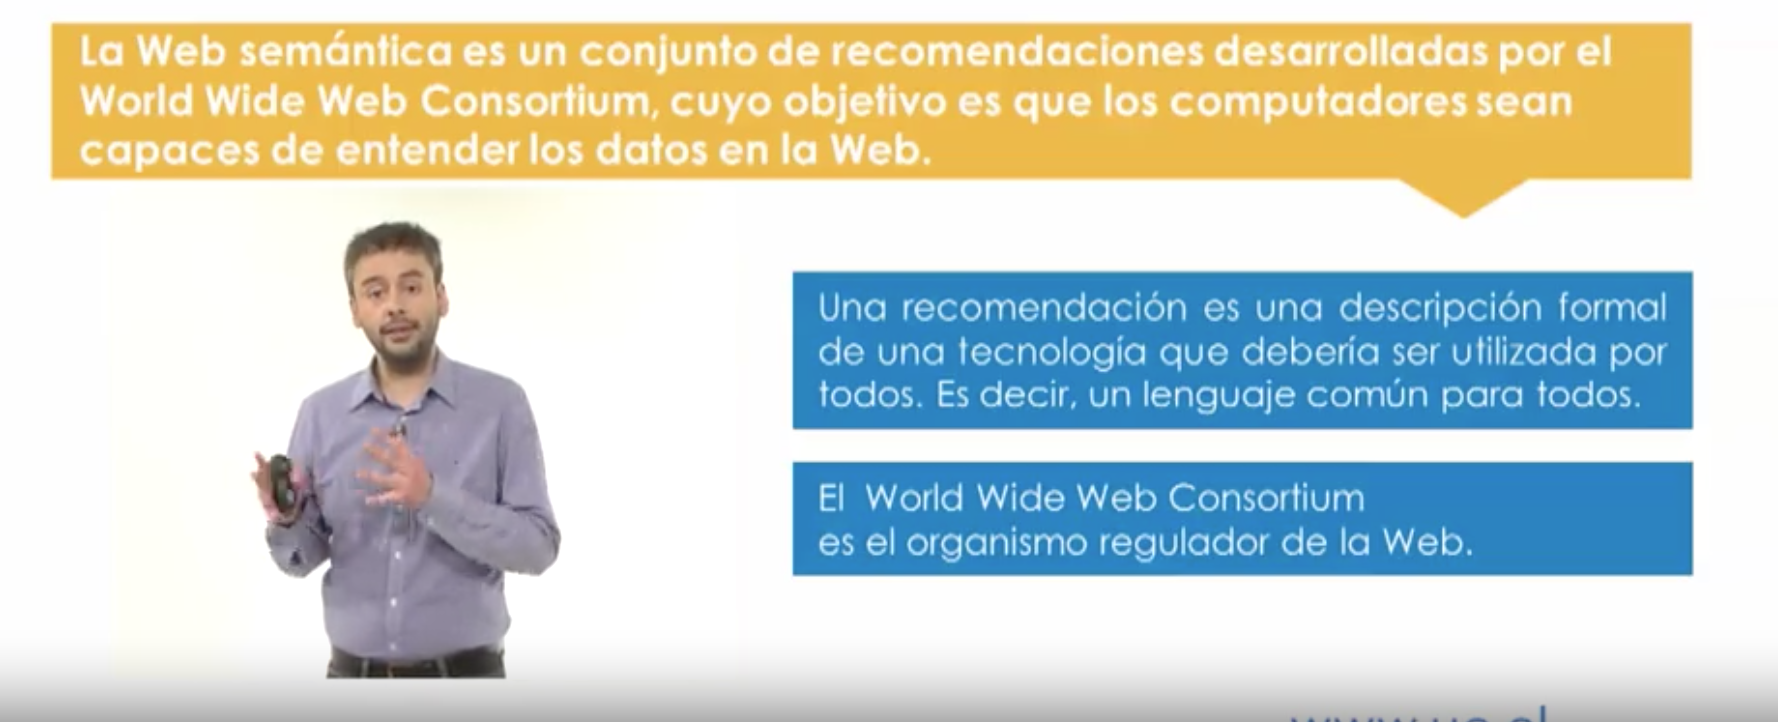
\includegraphics[height=4.5cm]{imagenes/capitulo3/8}
	\caption{}
\end{figure}

Han pasado más de diez años y es bien seguro que la Web ha revolucionado muchos aspectos de nuestras vidas cotidianas, pero la revolución que se preveía en el artículo del Scientific American todavía no se ha producido, por lo menos no en su totalidad. Sin embargo, la visión de una web semántica que describieron Berners-Lee y sus colaboradores desencadenó toda un línea de proyectos de investigación, y, precisamente, en octubre pasado se celebró en Bonn, Alemania, la 10ª edición del Congreso Internacional sobre la Web Semántica. Pero, ¿qué significa que la Web sea semántica? Y ¿en qué medida la semántica en la Web ya ha revolucionado o acabará por revolucionar Internet? % http://www.fgcsic.es/lychnos/es_es/articulos/construyendo_una_web_semantica

Ahora, ¿cuáles son esos estándares para la web? En la figura usted puede observar la pirámide de estándares que se está desarrollando para llevar a cabo esta web semántica. Y en esta pirámide en la parte inferior vemos los componentes más básicos, en la parte superior donde vemos el trust o el nivel de confianza ve uno en los niveles superiores. En este curso nos vamos a centrar en cuatro de estos componentes de esta pirámide que están marcados con colores. En primer lugar vamos a ver RDF, que es el lenguaje básico para especificar recursos de la web y sus relaciones, RDFS que nos permite decir un poco más vamos a hablar de este vocabulario, SPARQL que es este lenguaje de consulta que nos permite extraer información desde la web y finalmente OWL o este lenguaje que nos permite identificar ontologías.


El potencial de la web de datos, al igual que pasó con la web de documentos, reside en la participación a gran escala de numerosas personas y organizaciones en la publicación sistemática de datos en la Web, siguiendo las buenas prácticas de Linked Data. Es esta participación masiva, con un esfuerzo relativamente bajo, la que está detrás del éxito de la Web actual. La publicación de datos es solo una parte de lo que constituye la web de datos. La otra parte la forman las aplicaciones informáticas que nos proveen de los servicios para acceder, consultar, buscar y combinar los datos. Al igual que la web de documentos no nos sería de gran utilidad sin navegadores, buscadores o servicios de interacción social, las funcionalidades de la web de datos nos las dan las aplicaciones determinadas sobre los datos enlazados que utilizan leguajes específicos de consulta en repositorios RDF, tales como SPARQL, que se inspira en el leguaje SQL (Structured Query Language) de consulta de bases de datos tradicionales, pero ahora especialmente diseñado para ser ejecutado sobre la tecnología web. % http://www.fgcsic.es/lychnos/es_es/articulos/construyendo_una_web_semantica


 \begin{figure}[H]
	\centering
	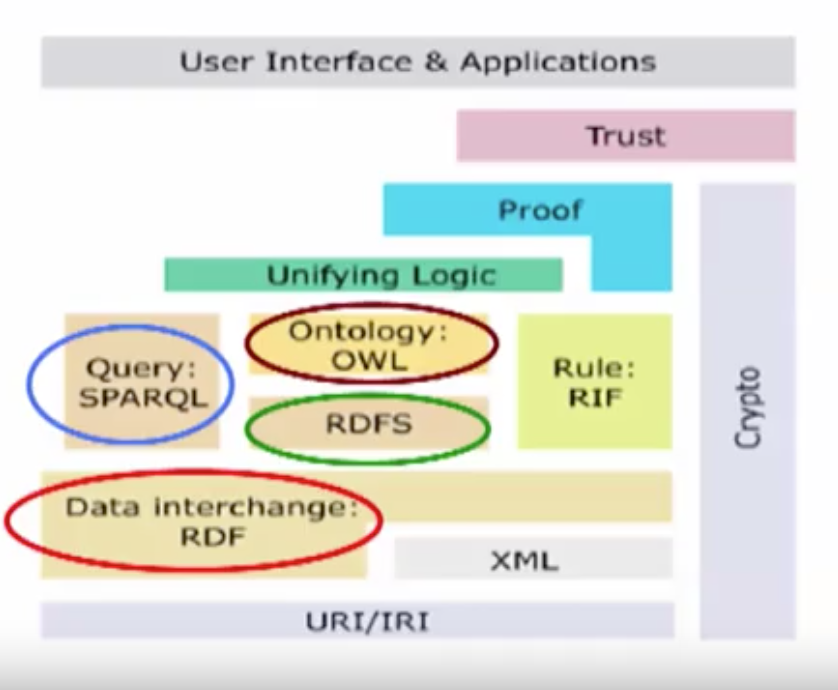
\includegraphics[height=4.5cm]{imagenes/capitulo3/9}
	\caption{}
\end{figure}

En resumen, ¿qué hemos visto hoy? Hemos visto que hay datos de todo tipo en la web, que son fácil acceso para las personas. Hemos visto que la cantidad de datos es tan grande que las personas no lo pueden manejar en su totalidad, son demasiados para que una persona simplemente pueda procesarlos por sí sola. También hemos visto que es difícil para un computador acceder a estos datos ya que no sabe como interpretarlos. La web de hoy en día está diseñada para ser leídas por personas, las páginas web están diseñadas para ser leídas por personas. ¿Sí? Y no está diseñada para que un computador las pueda leer de manera automática. Y finalmente la web semántica, que es el tema de este curso hemos visto que es un conjunto de recomendaciones para facilitar el acceso de los computadores a los datos. En particular, lo que queremos en este punto es tener el lenguaje que nos permita especificar los recursos que tenemos en la web, especificar las relaciones que tenemos entre ellos y también definir lenguajes que nos permitan extraer de manera automática de esta web.

\section{Arquitectura Web Semántica}

% % https://www.researchgate.net/figure/Figura-1-Arquitectura-de-la-web-semantica-Fuente-Tim-Berners-Lee_fig2_216537707


\section{¿Qué no es la Web Semántica?}


\section{Tecnologías de la Web Semántica}

\subsection{Metadatos explícitos}

Representación más fácilmente procesable por máquinas.

Metadata: data about data

Los metadatos representan parte del significado de los datos

La Web Semántica no se basa en la manipulación de texto, sino en metadatos procesables por las máquinas.

% XML
% RDF

% Ejemplo


\section{La web semántica en la práctica}

% http://www.fgcsic.es/lychnos/es_es/articulos/construyendo_una_web_semantica

Actualmente ya son numerosas las aplicaciones que de una forma u otra se basan en tecnologías semánticas para la Web. A continuación ilustraremos tres casos de naturaleza diversa para mostrar el potencial que todavía alberga la Web.

\textbf{Producción científica}. Uno de los pilares para el avance de la ciencia es la publicación de los resultados de la experimentación científica para que puedan ser contrastados y corroborados por la comunidad científica y para que a su vez puedan ayudar a avanzar en otras líneas de investigación. El portal GoPubMed, por ejemplo, ofrece un buscador semántico de publicaciones científicas en el área de la biomedicina. Está conectado con la Gene Ontology, una ontología que unifica y estructura la terminología sobre genes y productos génicos de un amplio número de organismos. Con GoPubMed se pueden localizar los textos relevantes para una búsqueda no únicamente por la ocurrencia de determinadas palabras clave sino por la relación semántica existente entre conceptos biomédicos. 

La publicación no solo de los resultados de una investigación sino también de los datos experimentales sobre los que se ha basado permitirá una mayor colaboración y transparencia en el ámbito de la investigación científica. Proyectos financiados por la Unión Europea, como OpenKnowledge o LiquidPub, han investigado formas novedosas de colaboración y publicación distribuida en la Web que apuntan a que vamos a ser testigos de un cambio importante en cómo se publican, se comparten y se diseminan los resultados científicos.

\textbf{Gobiernos abiertos}. Numerosos gobiernos nacionales están impulsando iniciativas de «gobierno abierto», haciendo públicos los conjuntos de datos en su posesión para promover la transparencia, aumentar la eficiencia administrativa y estimular el crecimiento económico. La combinación de estos datos mediante mashups –aplicaciones web que combinan datos y funcionalidades de diferentes fuentes– permite realizar consultas y presentar sus resultados de forma novedosa y creativa. En 2009, en una localidad del estado de Ohio, en Estados Unidos, un abogado creó un mashup que combinaba los datos públicos sobre la ubicación de las tuberías de agua corriente con los datos obtenidos del censo municipal sobre qué viviendas estaban habitadas por familias afroamericanas. El mapa resultante reveló que, en determinados barrios limítrofes, el ayuntamiento claramente discriminaba a los hogares afroamericanos. En consecuencia, un juez decretó una indemnización por daños y perjuicios.

% hablar sobre la página esa que tiene Londres - London Data store

\textbf{Colaboración popular masiva}. LinkedGeoData es una iniciativa para añadir una dimensión espacial a los datos publicados en la web semántica y se basa en la información recogida por el proyecto OpenStreetMap, un mapa mundial abierto al que cualquiera puede añadir datos, al estilo de Wikipedia. A finales del 2009 muy pocas áreas de la ciudad de Port-au-Prince en Haití estaban etiquetadas. Pero justo después del gran terremoto de enero de 2010, cuando se hicieron públicas imágenes de satélite del país, miles de personas estudiaron estas imágenes y comenzaron a anotar en el OpenStreetMap información detallada sobre las zonas devastadas: carreteras bloqueadas, edificios dañados, ubicación de campos de refugiados y hospitales de campaña, muelles en los que atracaban los barcos con ayuda humanitaria, etc. Todos estos datos fueron de gran utilidad para los equipos de rescate que sobre el terreno consultaban esta información con sus dispositivos móviles.



\subsection{Ontologías}

El término “Ontología” viene de la Filosofía: El estudio de la naturaleza de la existencia.

Tiene un significado distinto en Informática:

– Una ontología es una especificación formal y explícita de una conceptualización.

Proporcionan un entendimiento compartido de un dominio: interoperabilidad semántica.

– Solucionan diferencias en terminología.

– Hay que establecer correspondencias entre ontologías.

Útiles para organizar y navegar sitios Web.

% Hay tres tipo de ontologías

% Deberíamos ver como dar la definición de la ontología básica, y luego ver dicha definición para la Web Semántica

% Poner ejemplos de ontologías

% Existen ontologías geoespaciales y ontologías básicas, estaría bien centrarse en ambas

% Ver los estándares

%  Ejemplo

Hay varios lenguajes de ontología disponibles para codificar la ontología.


% Ontologías y razonamiento automatizado
% http://www.fgcsic.es/lychnos/es_es/articulos/construyendo_una_web_semantica
En último término, la visión de una web semántica, tal y como la plantearon Berners-Lee y sus colaboradores hace diez años, incluye también la posibilidad de razonar y sacar conclusiones lógicas de forma automatizada a partir de los datos publicados en la Web. Así pues, del hecho de que España comparta frontera con Francia y de que compartir frontera signifique que las regiones geográficas que constituyen estos países son contiguas, se debería poder deducir automáticamente que uno puede desplazarse de España a Francia por tierra sin tener que cruzar un tercer país. Esto, requiere que dispongamos de definiciones formales —es decir procesables por una computadora— de lo que significa la relación de contigüidad entre regiones espaciales y su relación con el desplazamiento continuo en regiones del espacio.

Esta información adicional que complementa los datos y con la cual se pueden deducir relaciones semánticas sin que estén explícitamente representadas en el conjunto de datos es lo que se llama una ontología. Habitualmente se trata de un conjunto de expresiones en un lenguaje formal basado en la lógica que describe con mayor o menor detalle los conceptos y sus interrelaciones de un área de conocimiento en particular (por ejemplo de la geografía en general o de la de España en particular). Para poder publicar y razonar con ontologías en la Web se recomienda utilizar el Web Ontology Language (OWL).

\subsubsection{OWL}


\subsection{Lógica e Inferencia}

La Lógica estudia los principios del razonamiento.

Los razonadores automáticos pueden deducir (inferir) conclusiones a partir de un conocimiento.

La lógica se puede usar a partir del conocimiento representado mediante ontologías para

– Descubrir nuevo conocimiento no expresado explícitamente. 
– Descubrir inconsistencias.

Poder expresivo vs. complejidad computacional:

– Cuanto más expresiva es una lógica, llegar a conclusiones puede ser más costoso computacionalmente.

Explicaciones: Expresión de los pasos de inferencia seguidos.

% Ejemplo inferencias

\subsection{Agentes}


Los Agentes trabajan de forma proactiva y autónoma.


Un agente personal en la Web Semántica:

– Recibirá tareas y preferencias de un usuario.

– Buscará información de fuentes Web, comunicándose con otros agentes.

– Comparará información sobre requerimientos de usuarios y preferencias para tomar decisiones.

– Dará respuestas al usuario.


\section{Lenguaje de marcado geográfico}

En literatura, se han desarrollado varios estándares útiles para facilitar el intercambio de datos espaciales. Por ejemplo, el archivo de datos geográficos (GDF) es un formato de archivo intercambiable para compartir datos geográficos. GDF está diseñado específicamente para el intercambio de datos espaciales para sistemas de transporte inteligente (ITS).

% aquí se debe de hablar de GML

% hablar sobre GDF y SDTS

% Extensible Markup Language (XML). 
% Resource Description Framework (RDF). 
% Web Ontology Language (OWL).

\section{XML}

Geography Markup Language (GML) es “una gramática XML escrita en XML Schema para el modelado, transporte y almacenamiento de información geográfica, incluidas las propiedades espaciales y no espaciales de las características geográficas”

\section{SVG}

Como su nombre lo indica, SVG es un gráfico vectorial, que es diferente de los formatos de imagen rasterizada, como GIF, JPEG y PNG. Como gráfico vectorial, SVG utiliza declaraciones matemáticas para describir las formas y los trazados de una imagen.\\

% hablar sobre la escalibilidad de SVG

Los datos GML se pueden transformar en formato SVG utilizando un procesador XSLT a través de la combinación con una hoja de estilo. XSLT (Transformaciones de lenguaje extensible de hojas de estilo) es un lenguaje para transformar documentos XML en otros documentos XML u otros objetos, como HTML para páginas web.

% limitaciones de SVG

\section{RDF}

\section{SPARQL}

\section{Ontologías}

% Hay tres tipo de ontologías

% Deberíamos ver como dar la definición de la ontología básica, y luego ver dicha definición para la Web Semántica

% Poner ejemplos de ontologías

% Existen ontologías geoespaciales y ontologías básicas, estaría bien centrarse en ambas

% Ver los estándares


Hay varios lenguajes de ontología disponibles para codificar la ontología.

\subsection{OWL}







\section{Servicios web geoespaciales}

Con el desarrollo de estándares abiertos, surgieron servicios web para la interoperabilidad de datos a través de la web. Los servicios web son componentes de software autocontenidos y autodescritos que pueden ser descubiertos e invocados por otros componentes de software a través de la web.



\section{Reglas del futuro}

% http://www.fgcsic.es/lychnos/es_es/articulos/construyendo_una_web_semantica

La web de datos, con sus vocabularios y ontologías, es un ente abierto y dinámico. Continuamente aparecen nuevos datos y nuevos enlaces entre ellos, mientras otros quedan obsoletos y se eliminan. Además, los servidores que hospedan estos datos a veces no están activos, bien porque han caído o bien porque están bajo mantenimiento. Eso implica una gran variabilidad semántica en los datos, por lo que hay que abordar los problemas que surgen cuando cambia el significado de un término, aparece una nueva terminología o surgen definiciones contradictorias. La publicación masiva de datos implica tener que preservar la privacidad de las personas e instituciones, garantizando que no sea posible deducir indirectamente determinada información confidencial. Además, el hecho de que cualquiera pueda publicar y enlazar datos en la web de datos implica que hay que tener en cuenta también aspectos sobre la procedencia de los datos, su calidad y la fiabilidad de las fuentes.

Todas estas son ricas áreas de investigación en las que aplicar técnicas de inteligencia artificial, como el razonamiento automático, el alineamiento semántico, los modelos computacionales de confiabilidad, la minería de datos para la preservación de la privacidad y el control de revelación de estadísticas. Pero, en última instancia, las posibilidades de esta web semántica están en las manos de los usuarios, que son los que generan los datos e idean los servicios que, como decía Tim Berners-Lee, harán realidad todo el potencial de la Web.

\section{Resumen del capítulo}

- Interoperabilidad de datos geoespaciales: integración y estandarización

- Dan problemas GDF y SDTS

- Ventajas del XML

- ¿Por qué usar XML?

- ¿Por qué es escalable SVG?

- Limitaciones SVG

Este capítulo presenta la información de fondo sobre la interoperabilidad de datos geoespaciales y las tecnologías más avanzadas para lograr la interoperabilidad de datos geoespaciales, como GML, SVG y servicios web geoespaciales. Aunque se han desarrollado muchas bases de datos de SIG, la interoperabilidad de los datos geoespaciales sigue siendo un desafío para la comunidad geoespacial. GML como formato estándar de intercambio de datos tiene como objetivo lograr el objetivo de la interoperabilidad de los datos al proporcionar mecanismos para compartir y reutilizar datos a nivel de características en la Web. Sin embargo, GML se ha diseñado para mantener el principio de separar el contenido de la presentación. Por lo tanto, se puede usar SVG para diseñar los datos GML para la presentación. Como gráfico vectorial, SVG puede mostrar mapas de alta calidad. Mientras que GML proporciona un medio para codificar y transportar características geoespaciales a XML, SVG proporciona un medio para mostrar estas características geoespaciales codificadas en GML en mapas vectoriales en la Web. Un tema de preocupación es cómo realizar colas y extraer características de la base de datos para responder a las solicitudes de los usuarios. Las especificaciones de implementación de servicios web geoespaciales desarrolladas por OGC cumplen esta función. Específicamente, (1) Web Feature Service (WFS) permite a un cliente recuperar, consultar y manipular datos geoespaciales a nivel de característica codificados en GML (Geography Markup Language) desde múltiples fuentes; (2) Web Map Service es capaz de crear y mostrar mapas que provienen simultáneamente de múltiples fuentes heterogéneas en un formato de imagen estándar; (3) el Servicio de cobertura web proporciona acceso a conjuntos potencialmente detallados y ricos de información geoespacial en formas que son útiles para la representación del lado del cliente, cobertura multivalor y aportes a modelos científicos y otros clientes; (4) Web Processing Service define reglas para estandarizar entradas y salidas (solicitudes y respuestas) de servicios de procesamiento geoespacial; (5) El Servicio de catálogos proporciona catálogos para servicios web de OGC y admite la capacidad de publicar y buscar colecciones de información descriptiva (metadatos) para datos, servicios y objetos de información relacionados. La arquitectura que hace uso completo de los servicios de catálogo web y otros servicios web, como OGC WFS, WMS, WCS y WPS, se denomina Arquitectura Orientada a Servicios (SOA). La SOA se aleja de los sistemas monolíticos hacia sistemas distributivos con componentes interoperables, y las implementaciones de la SOA pueden disminuir los problemas en la duplicación y el mantenimiento de los datos y modelos.











